% Build with latexmk -pdf icml2026.tex (includes BibTeX automatically).
\documentclass{article}

% Figures and typesetting: also recommended by the official ICML template.
\usepackage{microtype}
\usepackage{graphicx}
\usepackage{subcaption}
\usepackage{booktabs}
\usepackage{tikz}
\usetikzlibrary{arrows.meta}
% Figure-only font settings; the paper's main text remains in the ICML font.
\usepackage[type1,lining,tabular]{FiraSans}
\usepackage{sansmath}
\DeclareMathAlphabet{\mathbffira}{T1}{FiraSans-TLF}{b}{n}
\tikzset{every picture/.append style={execute at begin picture={\renewcommand{\sfdefault}{FiraSans-TLF}\fontfamily{FiraSans-TLF}\selectfont\sansmath\let\mathbf\mathbffira}}}

\usepackage[dvipsnames]{xcolor}
\usepackage{tcolorbox}
\usepackage{enumitem}
\definecolor{notegreen}{HTML}{56816B}
\definecolor{notebackground}{HTML}{F3F8F4}
\newtcolorbox{greenbox}[1]{%
  colback=notebackground, colframe=notegreen,
  colbacktitle=notegreen, coltitle=white,
  fonttitle=\fontfamily{FiraSans-TLF}\bfseries\selectfont,
  title={#1}, toptitle=5pt, bottomtitle=5pt,
  boxrule=0pt, sharp corners,
  boxsep=0pt, left=6pt, right=6pt, top=5pt, bottom=5pt,
  before skip=10pt, after skip=10pt
}
\usepackage{hyperref}
\newcommand{\theHalgorithm}{\arabic{algorithm}}

% Anonymous submission. Use [preprint] for a public draft or [accepted]
% for the camera-ready version. Keep the official style files unchanged.
\usepackage{icml2026}

% Useful packages from equivariant-sae-paper.
\usepackage{amsmath}
\usepackage{amssymb}
\usepackage{mathtools}
\usepackage{amsthm}
\usepackage{nicefrac}
\usepackage{multirow}
\usepackage{algorithm}
\usepackage{algorithmic}
\usepackage[capitalize,noabbrev]{cleveref}

% Reader-facing bibliography notes, on the next line without extra spacing.
\newcommand{\bibnote}[1]{\unskip\newline\textbf{\textbullet\ #1}}

\theoremstyle{plain}
\newtheorem{theorem}{Theorem}[section]
\newtheorem{lemma}[theorem]{Lemma}
\newtheorem{proposition}[theorem]{Proposition}
\theoremstyle{definition}
\newtheorem{definition}[theorem]{Definition}
\newtheorem{assumption}[theorem]{Assumption}

% Same optional author-comment workflow as equivariant-sae-paper.
\newif\ifshowComments
\showCommentsfalse % Change to \showCommentstrue while drafting.
\ifshowComments
\newcommand{\ee}[1]{{\color{blue}#1}}
\newcommand{\al}[1]{{\color{red}#1}}
\else
\newcommand{\ee}[1]{}
\newcommand{\al}[1]{}
\fi

\icmltitlerunning{Latent Physics in AI Weather Models}

\begin{document}

\twocolumn[
  \icmltitle{Latent Physics in AI Weather Models}
  % Replace these placeholders before using preprint or accepted mode.
  \begin{icmlauthorlist}
    \icmlauthor{Author Name}{institution}
  \end{icmlauthorlist}
  \icmlaffiliation{institution}{Department, University, City, Country}
  \icmlcorrespondingauthor{Author Name}{author@example.com}
  \vskip 0.3in
]

\printAffiliationsAndNotice{}

\begin{abstract}
  % Abstract goes here.
\end{abstract}

\section{Introduction} \label{sec:introduction}

\section{Background} \label{sec:background}

\subsection{Problem Setup of Weather Modeling}

\subsection{Aurora}

\section{Related Work}

\subsection{Weather Interp}

Comprehensive list of activation-based interp of weather models.

\section{Probing}

\begin{figure*}[t!]
  \centering
  \resizebox{\textwidth}{!}{%
    % Native TikZ schematic; weather panels are rendered from cached ERA5 data.
\begin{tikzpicture}[
  x=1cm,y=1cm,font=\footnotesize,
  flow/.style={-{Latex[length=2mm]},draw=black!65,line width=.7pt},
  detail/.style={draw=black!35,dashed,line width=.6pt},
  box/.style={draw=black!35,rounded corners=2pt,align=center,fill=white},
  labeltext/.style={align=center,text=black!75}
]
\definecolor{probeBlue}{HTML}{356A91}
\definecolor{probeOrange}{HTML}{C87536}
\path[use as bounding box] (0,0) rectangle (17.1,7.9);
\node[fill=black,text=white,minimum size=.38cm,inner sep=0pt,font=\small\bfseries] at (.34,7.55) {A};
\node[anchor=west,font=\small\bfseries,inner sep=0pt] at (.65,7.55) {Probing Aurora's backbone};
\draw[black,line width=.8pt] (.15,7.24) -- (16.950000000000003,7.24);

% Main forward pass.
\node[font=\small\bfseries] at (1.6,6.85) {ERA5 inputs};
\foreach \hour/\base/\timelabel in {12/5.65/{$t-6$ h},18/3.95/{$t$}} {
  % Staggered cards show distinct fields at each input time.
  \foreach \field/\dx/\dy/\fieldlabel in {
    q850/.48/.48/{Humidity, 850 hPa},10u/.24/.24/{Zonal wind, 10 m},2t/0/0/{Temperature, 2 m}} {
    \begin{scope}[shift={({1.25+\dx},{\base+\dy})}]
      \node[inner sep=0] at (0,-.08) {\includegraphics[width=1.96cm]{figures/era5_\field_\hour.png}};
    \end{scope}
  }
  \node[font=\scriptsize,anchor=west] at (2.95,{\base+.5}) {\timelabel};
}
\node[box,fill=probeBlue!7,minimum width=2.4cm,inner xsep=1.5mm,minimum height=1.25cm] (aurora) at (4.875,5.35)
  {\textbf{Aurora 1.5}\\Frozen parameters};
\draw[flow] (3.05,5.35) -- (aurora.west);
\draw[flow] (aurora.east) -- (6.7,5.35);
\node[font=\small\bfseries] at (9.1,6.85) {Backbone tensor};
% Rectangular tensor: longitude horizontally, latitude in depth, latent levels vertically.
\begin{scope}[shift={(7.5,4.4)}]
  \begin{scope}[opacity=.35]
  \filldraw[fill=probeBlue!10,draw=probeBlue!70,line width=.6pt]
    (0,1.6) -- (.8,2.2) -- (3.2,2.2) -- (2.4,1.6) -- cycle;
  \filldraw[fill=probeBlue!19,draw=probeBlue!70,line width=.6pt]
    (2.4,0) -- (3.2,.6) -- (3.2,2.2) -- (2.4,1.6) -- cycle;
  \foreach \i in {1,...,5} {
    \draw[probeBlue!45,line width=.3pt] ({.4*\i},1.6) -- ({.4*\i+.8},2.2);
  }
  \foreach \i in {1,2,3} {
    \draw[probeBlue!45,line width=.3pt] (2.4,{.4*\i}) -- (3.2,{.4*\i+.6});
    \draw[probeBlue!60,line width=.4pt] ({.2*\i},{1.6+.15*\i}) -- ({2.4+.2*\i},{1.6+.15*\i});
    \draw[probeBlue!60,line width=.4pt] ({2.4+.2*\i},{.15*\i}) -- ({2.4+.2*\i},{1.6+.15*\i});
  }
  \filldraw[fill=probeBlue!5,draw=probeBlue!70,line width=.6pt] (0,0) rectangle (2.4,1.6);
  \draw[step=.4,probeBlue!35,line width=.3pt] (0,0) grid (2.4,1.6);
  \end{scope}
  % Selected token occupies one cell along each of the three tensor axes.
  \filldraw[fill=probeOrange!25,draw=probeOrange,line width=.8pt]
    (.8,1.2) -- (1,1.35) -- (1.4,1.35) -- (1.2,1.2) -- cycle;
  \filldraw[fill=probeOrange!65,draw=probeOrange,line width=.8pt]
    (1.2,.8) -- (1.4,.95) -- (1.4,1.35) -- (1.2,1.2) -- cycle;
  \filldraw[fill=probeOrange!45,draw=probeOrange,line width=.9pt]
    (.8,.8) rectangle (1.2,1.2);
\end{scope}
\node[rotate=90,font=\scriptsize,fill=white,inner sep=1pt] at (6.97,5.2) {Latent level $l$};
\foreach \l in {0,1,2,3} {
  \node[font=\scriptsize,anchor=east,inner sep=1pt] at (7.47,{4.6+.4*\l}) {$\l$};
}
\node[font=\scriptsize,rotate=36.87,inner sep=1pt] at (10.45,4.45) {$H$};
\draw[detail] (8.3,5.2) -- (6.4,3.14);
\draw[detail] (8.7,5.2) -- (9.25,3.14);
% Keep the spatial-axis label clear of the close-up guides.
\node[font=\scriptsize,fill=white,inner sep=1pt] at (8.7,3.96) {$W$};
\node[font=\small\bfseries] at (15.05,6.85) {ERA5 target};
\node[inner sep=0] at (15.05,5.65) {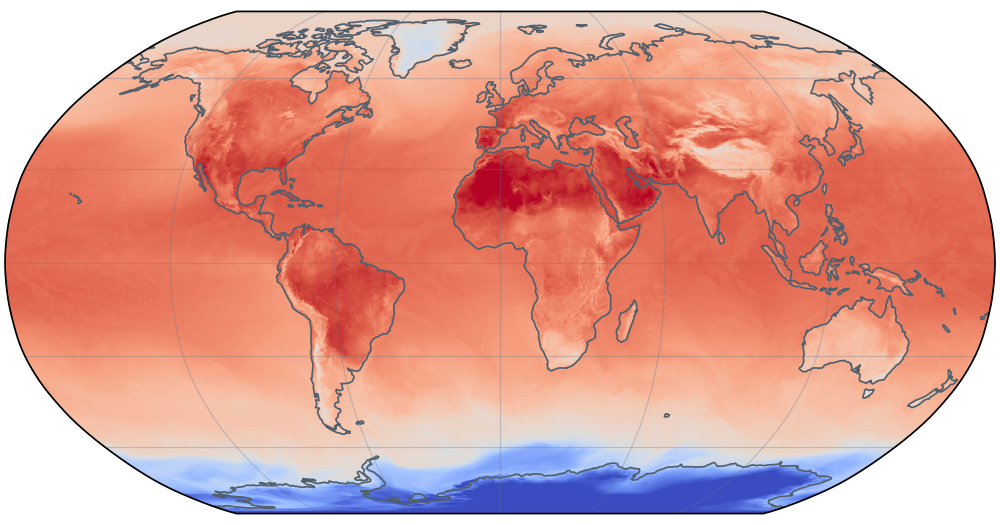
\includegraphics[width=3.35cm]{figures/era5_2t_18.png}};
\node[labeltext] (targetlabel) at (15.05,4.5) {$\mathbf{Y}_c$ at $t+\tau$};

% One-token close-up. A selected channel set is fitted separately per j.
\draw[rounded corners=3pt,draw=black!20,fill=black!1] (.15,.12) rectangle (16.95,3.12);
\node[anchor=west,font=\bfseries,text=probeOrange] at (.4,2.85) {One spatial token, one latent level};
\node[labeltext] at (2.1,2.25) {$D$ activation channels};
\foreach \i in {0,...,11} {
  \filldraw[fill=black!9,draw=white,line width=.6pt] ({.55+.26*\i},1.15) rectangle ++(.26,.55);
}
\foreach \i in {1,4,8} {
  \filldraw[fill=probeOrange!65,draw=white,line width=.6pt] ({.55+.26*\i},1.15) rectangle ++(.26,.55);
}
\node[labeltext,font=\scriptsize] at (2.1,.72) {Select $k$, then standardize\\Separately for each position $j$};
\node[box,draw=probeBlue!70,fill=probeBlue!6,minimum width=3.4cm,minimum height=.85cm] (readout) at (6.5,1.42)
  {\textbf{Linear readouts}\\$\mathbf{w}_{c,j}^{\top}\mathbf{h}_{c,j}(n)+\beta_{c,j}$};
\node[labeltext,font=\scriptsize] at (6.5,.55) {One readout per patch cell\\Weights shared across spatial tokens};
\draw[flow,shorten <=1mm,shorten >=1mm] (3.67,1.42) -- (readout.west);
\draw[flow,shorten <=1mm,shorten >=1mm] (readout.east) -- (9.7,1.42);
\node[labeltext] at (10.45,2.55) {Predicted ERA5 patch};
\foreach \i in {0,...,3} {
  \foreach \j in {0,...,3} {
    \filldraw[fill=probeBlue!9,draw=white,line width=.7pt] ({9.7+.36*\i},{.72+.36*\j}) rectangle ++(.36,.36);
  }
}
\draw[draw=probeBlue!65,line width=.5pt] (9.7,.72) rectangle (11.14,2.16);
\filldraw[fill=probeOrange!45,draw=probeOrange,line width=.8pt] (10.06,1.44) rectangle ++(.36,.36);
\node[font=\scriptsize] at (10.24,1.62) {$j$};
\node[labeltext,font=\scriptsize] at (10.45,.4) {$\widehat{\mathbf{Y}}_c(n,j)$, schematic};
\node[box,minimum width=3.1cm,minimum height=.85cm] (eval) at (15.05,1.42)
  {\textbf{Compare with ERA5}\\MAE, RMSE, spatial $\rho$};
\draw[flow,shorten <=1mm,shorten >=1mm] (11.14,1.42) -- (eval.west);
\draw[flow,shorten <=2mm,shorten >=1mm] (targetlabel.south) -- (eval.north);
\end{tikzpicture}
\hspace{5mm}%
    % Spatial extents use relative scales 1, 1/2, 1/4; latent height stays fixed.
\begin{tikzpicture}[x=1cm,y=1cm,font=\footnotesize]
\definecolor{stageBlue}{HTML}{356A91}
\definecolor{stageOrange}{HTML}{C87536}
\path[use as bounding box] (0,0) rectangle (6.6,7.9);
\node[fill=black,text=white,minimum size=.38cm,inner sep=0pt,font=\small\bfseries] at (.34,7.55) {B};
\node[anchor=west,font=\small\bfseries,inner sep=0pt] at (.65,7.55) {Stage outputs and ERA5 patches};
\draw[black,line width=.8pt] (.15,7.24) -- (6.449999999999999,7.24);
\foreach \stage/\ratio/\patch/\row in {
 E0/1/4/0,E1/.5/8/1,E2/.25/16/2,
 D0/.25/16/3,D1/.5/8/4,D2/1/4/5} {
  \pgfmathsetmacro{\yy}{6.35-1.10*\row}
  \pgfmathsetmacro{\ww}{2.08*\ratio}
  \pgfmathsetmacro{\dx}{.64*\ratio}
  \pgfmathsetmacro{\dy}{.48*\ratio}
  \pgfmathtruncatemacro{\cols}{16*\ratio}
  \pgfmathtruncatemacro{\depth}{4*\ratio}
  \pgfmathsetmacro{\leftedge}{2.05-(\ww+\dx)/2}
  \pgfmathsetmacro{\base}{\yy-(.56+\dy)/2}
  \node[font=\bfseries,anchor=west] at (.05,\yy) {\stage};
  \begin{scope}[shift={(\leftedge,\base)}]
    \filldraw[draw=stageBlue!40,fill=stageBlue!4,line width=.45pt]
      (0,.56) -- (\dx,{.56+\dy}) -- ({\ww+\dx},{.56+\dy}) -- (\ww,.56) -- cycle;
    \filldraw[draw=stageBlue!40,fill=stageBlue!9,line width=.45pt]
      (\ww,0) -- ({\ww+\dx},\dy) -- ({\ww+\dx},{.56+\dy}) -- (\ww,.56) -- cycle;
    \foreach \i in {1,...,\cols} {
      \draw[stageBlue!22,line width=.25pt] ({.13*\i},.56) -- ({.13*\i+\dx},{.56+\dy});
    }
    \foreach \i in {1,...,\depth} {
      \draw[stageBlue!25,line width=.25pt] ({.16*\i},{.56+.12*\i}) -- ({\ww+.16*\i},{.56+.12*\i});
      \draw[stageBlue!25,line width=.25pt] ({\ww+.16*\i},{.12*\i}) -- ({\ww+.16*\i},{.56+.12*\i});
    }
    \foreach \i in {1,2,3} {
      \draw[stageBlue!25,line width=.25pt] (\ww,{.14*\i}) -- ({\ww+\dx},{.14*\i+\dy});
    }
    \filldraw[draw=stageBlue!40,fill=stageBlue!2,line width=.45pt] (0,0) rectangle (\ww,.56);
    \foreach \i in {1,2,3} {\draw[stageBlue!22,line width=.25pt] (0,{.14*\i}) -- (\ww,{.14*\i});}
    \foreach \i in {1,...,\cols} {\draw[stageBlue!22,line width=.25pt] ({.13*\i},0) -- ({.13*\i},.56);}
    \pgfmathsetmacro{\xx}{\ww/2-.13}
    \filldraw[fill=stageOrange!25,draw=stageOrange,line width=.4pt]
      (\xx,.42) -- ({\xx+.16},.54) -- ({\xx+.29},.54) -- ({\xx+.13},.42) -- cycle;
    \filldraw[fill=stageOrange!65,draw=stageOrange,line width=.4pt]
      ({\xx+.13},.28) -- ({\xx+.29},.40) -- ({\xx+.29},.54) -- ({\xx+.13},.42) -- cycle;
    \filldraw[fill=stageOrange!45,draw=stageOrange,line width=.4pt] (\xx,.28) rectangle ({\xx+.13},.42);
  \end{scope}
  \draw[-{Latex[length=1.4mm]},black!50,line width=.5pt] (3.6,\yy) -- (4.4,\yy);
  \node[inner sep=0] at (5.15,\yy) {\includegraphics[height=.94cm]{figures/era5_patch_\patch.png}};
}
\end{tikzpicture}
%
  }
  \caption{Probing Aurora's backbone representations. \textbf{(A)} ERA5 surface and atmospheric inputs at $t-6$ h and $t$, together with static fields, produce the stage activations. Atmospheric inputs include all 13 pressure levels. For each within-patch position $j$, we select $k$ channels from one token and fit a linear readout, sharing its weights across spatial tokens. Repeating this readout over the grid reconstructs the target field for evaluation against ERA5. The close-up shows a schematic $4\times4$ patch; larger patches use the same procedure. Actual ERA5 maps of 2 m temperature, 10 m zonal wind, and 850 hPa specific humidity from 6 August 2020 at 12:00 and 18:00 UTC illustrate the stacked inputs; the target example uses $\tau=0$. \textbf{(B)} Relative spatial dimensions are shown at each stage, with a constant four-level height, and the corresponding ERA5 footprint on the same geographic crop. Tensor grids are schematic; patch outlines follow the actual $0.25^\circ$ grid.}
  \label{fig:probing-setup}
\end{figure*}

We want to evaluate what information is linearly decodable from the residual stream of Aurora's backbone. We use linear probes: ridge regression \citep{hoerl1970ridge} to predict ERA5 fields and other quantities derived from the fields. Fundamental questions:
\begin{itemize}
  \item What information is or is not linearly decodable from Aurora's residual stream?
  \item How are different quantities geometrically related? Why?
\end{itemize}
Depending on the results these may support a \textit{distributed linear representation hypothesis} for Aurora, where physical quantities can be read linearly from the residual stream but not from individual neurons (hence \textit{distributed}).

\begin{greenbox}{Probing Takeaways}
  \begin{itemize}[leftmargin=*, labelindent=0pt]
    \item Aurora's latent levels roughly correspond in order to atmospheric pressure levels.
    \item The results support \textit{distributed linear representations}: much physical information can be read linearly from the residual stream, but not from individual or only a few neurons.
    \item Despite distributed representations, full-width probes concentrate importance on few neurons on average.
    \item Input fields can more easily be decoded from earlier layers and output (+6h) fields from the later layers. Middle layers are best for further ($>$ 6h) lead times.
  \end{itemize}
\end{greenbox}

\subsection{Training Setup}

We use bold symbols for vectors and fields (including activation tensors), and non-bold symbols for scalars.

\textbf{Targets.} We use the ERA5 ($1440 \times 721$ longitude--latitude grid, i.e. $0.25^\circ$) \citep{hersbach2020era5} fields as the probe targets. The evaluation grid is $720 \times 1440$ in latitude--longitude order. Surface fields: 2m temperature, 10m zonal and meridional wind, mean sea-level pressure, total column water vapor, and total cloud cover. Atmospheric fields (each at 250, 500, 700, 850 hPa): temperature, zonal and meridional wind, geopotential, and specific humidity. In addition to these fields directly provided in ERA5, we compute these atmospheric fields based on the ERA5 fields: wind speed, relative vorticity, and relative humidity.

\textbf{Inputs.} Inputs are the residual stream activations from the six stage outputs from the Aurora backbone. The full latent tensor at the end of a stage is of size $H \times W \times 4 \times D$ with a $H \times W$ spatial grid at four latent levels and $D$ channels per token. The latent levels do not have direct physical counterparts, but we can trace each latent token back to an ERA5 patch, although the latent tokens naturally contain information from surrounding patches as well as a result of attention and merge/split operations of the UNet transformer. Table \ref{tab:backbone_stages} shows the size of the spatial grid at each stage and the corresponding ERA5 patch size.

\begin{table}[t!]
  \caption{Spatial resolution and channel counts of Aurora's encoder (E) and decoder (D) stages. Grid dimensions are latitude $\times$ longitude; positions per token describe the probe output layout.}
  \label{tab:backbone_stages}
  \centering
  \small
  \setlength{\tabcolsep}{0pt}
  \begin{tabular*}{\columnwidth}{@{\extracolsep{\fill}}lcrc@{}}
    \toprule
    \textbf{Stage} & \textbf{Spatial grid} & \textbf{Channels} & \textbf{ERA5 patch size} \\
    \midrule
    E0 & $180 \times 360$ & 512 & $4 \times 4$ \\
    E1 & $90 \times 180$ & 1,024 & $8 \times 8$ \\
    E2 & $45 \times 90$ & 2,048 & $16 \times 16$ \\
    \midrule[0.3pt]
    D0 & $45 \times 90$ & 2,048 & $16 \times 16$ \\
    D1 & $90 \times 180$ & 1,024 & $8 \times 8$ \\
    D2 & $180 \times 360$ & 512 & $4 \times 4$ \\
    \bottomrule
  \end{tabular*}
\end{table}

To evaluate how distributed the representations are, we vary $k \in \{1,4,16,32,64,128,256,D\}$: the input dimension of a probe. For each target and Aurora stage, we only select the $k$ neurons with the largest squared Pearson correlation coefficient with the target.

We sample initializations at 00:00 UTC every three days starting on January 1 each year, resulting in 122 initializations per year. We use one year (2017) to select the top-$k$ neurons, three years (2018-2020) for training, and one year (2021) for evaluation.

\textbf{Probes.} Each latent token corresponds to multiple ERA5 cells rather than a single scalar, so we fit separate probes for each ERA5 cell a token corresponds to. These probes are shared between the latent tokens at the same latent level and stage. So e.g. for one target field with the E2 stage as the inputs, we fit $16 \times 16 \times 4 = 1,024$ probes.

We fit probes separately for each target quantity $q$, pressure level $p$ (for atmospheric targets), backbone stage $s$, latent level $l$, lead time $\tau \in \{0,6,12,18,24\}$ hours, and channel count $k$. We denote this combination by $c=(q,p,s,l,\tau,k)$.

Let $n$ index a date--token pair and $j$ a position within its ERA5 patch. The target field $\mathbf{Y}_c$ is arranged so that $\mathbf{Y}_c(n,j)$ is the target at that position and time $t_n+\tau$. The probe predicts
\begin{equation}
  \widehat{\mathbf{Y}}_c(n,j)
  = \mathbf{w}_{c,j}^{\top}\mathbf{h}_{c,j}(n)+\beta_{c,j}.
\end{equation}
Here $\mathbf{h}_{c,j}(n)\in\mathbb{R}^k$ contains the $k$ selected, standardized channels from $\mathbf{h}_l$ at stage $s$, with all lead times using activations from the same initial forward pass. The weights and intercept are shared across dates and spatial tokens.

For each $c$ and $j$, we fit ridge regression:
\begin{equation} \label{eq:ridge}
  \begin{aligned}
    \min_{\mathbf{w}_{c,j},\beta_{c,j}}\;&
    \sum_{n\in\mathcal{T}}
    \bigl(\mathbf{Y}_c(n,j)-\widehat{\mathbf{Y}}_c(n,j)\bigr)^2 \\
    &+\alpha\lVert\mathbf{w}_{c,j}\rVert_2^2.
  \end{aligned}
\end{equation}
Here $\mathcal{T}$ contains the training date--token pairs. We select $\alpha$ separately for each readout by generalized cross-validation on the training data; the intercept is unpenalized.

\textbf{Evaluation}. We follow the setup in \citep{lehmannFinetuningWeatherFoundation2025} and evaluate the probes using three metrics at each evaluation date: mean absolute error (MAE), root mean squared error (RMSE), and spatial Pearson correlation. For a fixed condition $c$ and evaluation date $t$, all sums below run over date--token pairs $n$ with $t_n=t$ and all within-patch positions $j$:
\begin{align}
  \mathrm{MAE}_{c,t}
  &=\frac{\sum_{n,j}|\mathbf{Y}_c(n,j)-\widehat{\mathbf{Y}}_c(n,j)|}
  {720\times1440} \\
  \mathrm{RMSE}_{c,t}
  &=\sqrt{\frac{\sum_{n,j}\bigl(\mathbf{Y}_c(n,j)-\widehat{\mathbf{Y}}_c(n,j)\bigr)^2}
  {720\times1440}} \\
  \rho_{c,t}
  &=\frac{\sum_{n,j}\delta\mathbf{Y}_c(n,j)\,
  \delta\widehat{\mathbf{Y}}_c(n,j)}
  {\sqrt{\sum_{n,j}\delta\mathbf{Y}_c(n,j)^2}
  \sqrt{\sum_{n,j}\delta\widehat{\mathbf{Y}}_c(n,j)^2}}
\end{align}
where $\delta\mathbf{Y}_c(n,j)$ and $\delta\widehat{\mathbf{Y}}_c(n,j)$ denote deviations from each field's spatial mean at date $t$.

\subsection{Higher (lower) latent levels correspond to higher (lower) pressure levels }

\begin{figure}[t!]
  \centering
  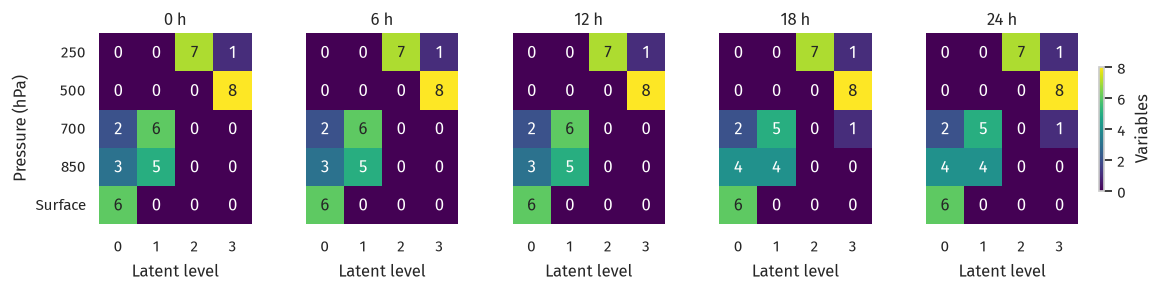
\includegraphics[width=\linewidth]{results/latent_pressure.png}
  \caption{Number of target fields from each pressure level that are best predicted from a certain latent level in the backbone. Best means the latnet level with the max pearson averaged between pretrained and random model probes.}
  \label{fig:latent_pressure}
\end{figure}

Figure \ref{fig:latent_pressure}: target fields at which pressure level can best be predicted by each latent level? By Aurora's design we expect that higher latents levels correspond to higher altituted (lower pressure). This generally holds. Latent 0 is the best for all six surface fields; for 850 and 700 hPa the first two latents always win, and for 500 and 250 hPa the last two latents win. This supports that information for the higher/lower altitudes is more easily readable from higher/lower latent levels.

\textbf{\color{orange} From now on we only report results from the best latent level for each target.}

\subsection{Probes support distributed linear representations}

\begin{figure}[t!]
  \centering
  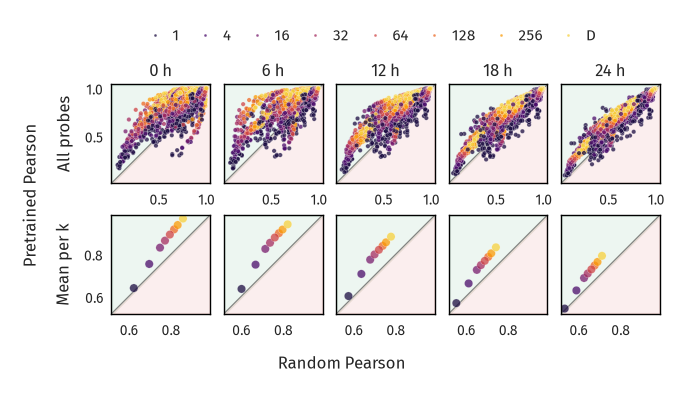
\includegraphics[width=\linewidth]{results/pretrained_v_random_scatter.png}
  \caption{Pearson of probes trained over pretrained and random model activations.}
  \label{fig:pretrained_v_random_scatter}
\end{figure}

Figure \ref{fig:pretrained_v_random_scatter}: compares the Pearson coeffs of probes trained over pretrained and random models across different $k$ values and lead times. 1) Probes over the pretrained model are usually more accurate. 2) Average performance tends to drop with larger lead times. 3) Larger $k$ leads to better performance, and $k=1$ probes are very similar between the pretrained and random models. These support that much information is linearly readable from the activations, but generally not from individual neurons.

Figure \ref{fig:probe_heatmaps} shows the RMSE gain observed by probing the pretrained model v the random init model for different $k$ values and lead times. The $u$ field is more easily accessible in the pretrained model across all combinations, whereas for total column water vapor (TCWV) the gain is more often negative than positive except when $k=D$. This means the tcwv field is no more linearly accessible from the pretrained model activations than from the random model activations.

Interestingly for the D1 layer, the gan is positive for small $k$ but negative for large $k$ across all lead times. This might mean that tcwv is particularly important for the final layer, or is passed directly from the inputs to the final layer through skip connections.

Similarly for the mean sea-level pressure (MSL), the gain is negative in the intermediate layer when $k$ is small and becomes positive only with large $k$, which might indicate that the pretrained model mostly learns to route the MSL-relevant information around those layers, and that they do not play a particularly important role for the computation in those layers.

We should be careful that red in these plots does not mean that the information is not present at all, but only that it is not more easily readable than from the activations of a randomly init model.

\subsection{Full-width probes are ``sparse"}

\begin{figure}[t!]
\centering
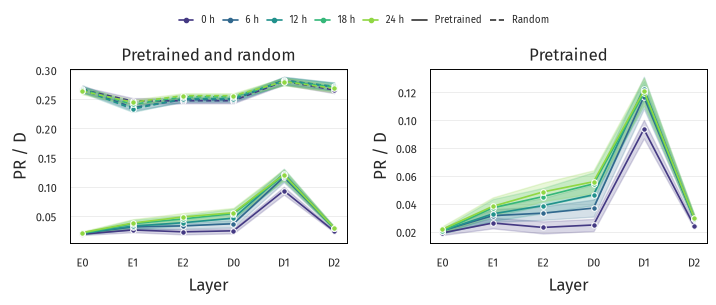
\includegraphics[width=\linewidth]{results/probe_particip_ratio.png}
\caption{Participation ratio of pretrained and random models at different layers and lead times.}
\label{fig:probe_particip_ratio}
\end{figure}

For each spatial position, we compute a full-width ($k=D$) probe's weight participation ratio as
$
\text{PR}(\mathbf{w})
=
\frac{1}{D} \left( \sum_i \mathbf{w}_i^2 \right)^2 / \sum_i \mathbf{w}_i^4
$. This is a way of quantifying how many of the neurons are ``important'' to the probe. PR closer to 1 means most neurons carry equal amount of weight, while PR closer to 0 means only a small fraction of neurons dominate.

Figure \ref{fig:probe_particip_ratio} shows that 1) PR values are significantly lower for the pretrained model probes than the random model probes (around 0.05-0.1 vs 0.25-0.3), and specifically for the pretrained model probes, 2) input probes (lead time = 0) consistently have smaller PRs with the PRs roughly increasing with lead time. These mean the input information is more easily readable from the Aurora backbone, and lead times further away require more neurons, perhaps becaus the probes are picking up on basic correlations between the quantities encoded across different neurons to predict future quantities (?).

There is also a noticeable spike for the D1 layer but we have no explanation right now for why.

\subsection{Future timesteps can be decoded more easily from later layers}

\begin{figure*}[t!]
\centering
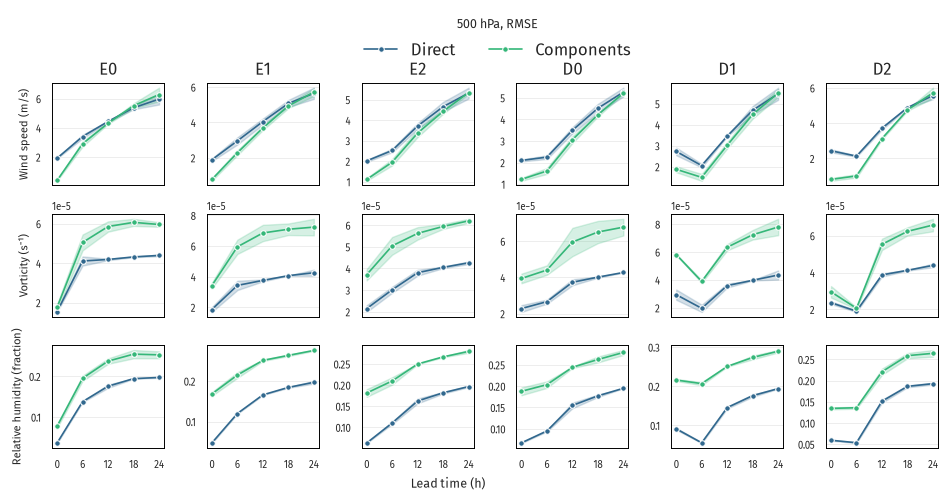
\includegraphics[width=0.9\linewidth]{results/probe_direct_v_derived.png}
\caption{RMSE for fields derived from ERA5 fields when directly probed and computed from the predictions of component probes.}
\label{fig:probe_direct_v_pretrained}
\end{figure*}

\begin{figure}[t!]
\centering
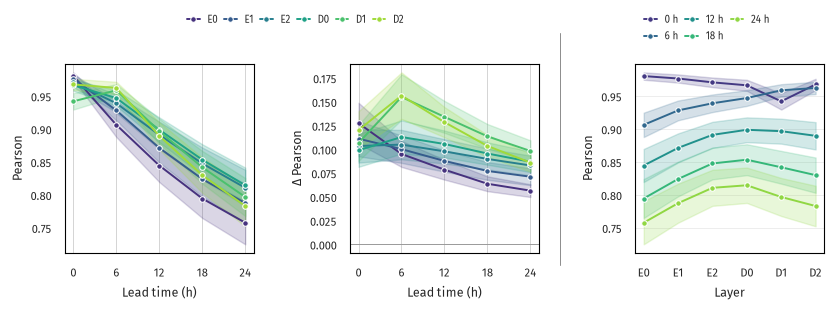
\includegraphics[width=\linewidth]{results/probe_layer_leadtime.png}
\caption{Pretrained model probe pearsons and gain vs the random model across different layers and lead times.}
\label{fig:probe_layer_leadtime}
\end{figure}

Figure \ref{fig:probe_layer_leadtime} shows the pearson coeffs of the pretrained model probes, and the difference between the pretrained and random init model, averages across all probe targets for the full-width probes. 1) the input fields (lead time 0) are most easily recovered from the first layer unsurprisingly, 2) the output fields (lead time 6 hrs) are most easily recovered from the last two layers which is also not surprising, and 3) the middle two layers E2 and D0 have maintain the highest absolute pearson for later lead times beyond 6 hrs, and D1 also results in the largest gain over the random model. This suggests that the early layers are very close to the input state, the later layers to the output state, and the middle layers are where the more general/informative processing happens.

The panel to the side of Figure \ref{fig:probe_layer_leadtime} also supports this -- the middle layers perform the best for the lead times > 6 hrs, while the 0h and 6h curves follow different patterns.

\subsection{For derived fields (not ERA5-provided), computing from component probes can outperform direct probing}

We compute the wind speed ($s$), relative vorticity ($\zeta$), and relative humidity (RH) fields from the ERA5-provided fields as follows:
\begin{align}
s &= \sqrt{u^2 + v^2} \quad (\text{m/s}) \\
\zeta &= \frac{\partial v}{\partial x} - \frac{\partial u}{\partial y} \quad (\text{s}^{-1}) \\
\text{RH} &\approx \frac{q}{q_s(T, p)} \quad (\text{no unit})
\end{align}
and we compare linear probing directly for these fields with computing them from the probes for their components; e.g. using the $u$ and $v$ probes separately to compute the wind speed.

Figure \ref{fig:probe_direct_v_pretrained} shows the resulting RMSEs for these fields at 500 hPa for different layers and lead times. For wind speed, using the component probes tends to outperform direct probing especially at small lead times. However, for relative vorticity and relative humidity direct probing is better.

Not clear if there is a global explanation for this, but:
\begin{itemize}
\item It makes sense for wind speed because using the components, we can explicitly compute the nonlinear operation which a linear probe might struggle to capture.
\item Vorticity is linear in its components so a linear probe might work, and the prediction errors in the individual components might amplify through differentation.
\item Harder to reason about for relative humidity, but the division might likewise amplify small prediction errors?
\end{itemize}

\begin{figure*}[t!]
\centering
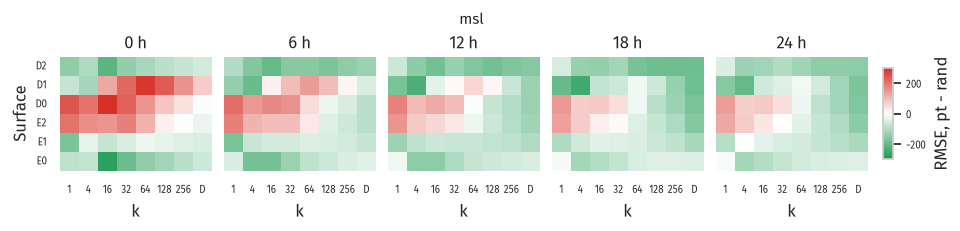
\includegraphics[width=\textwidth]{results/probe_heatmap_msl.png}\par
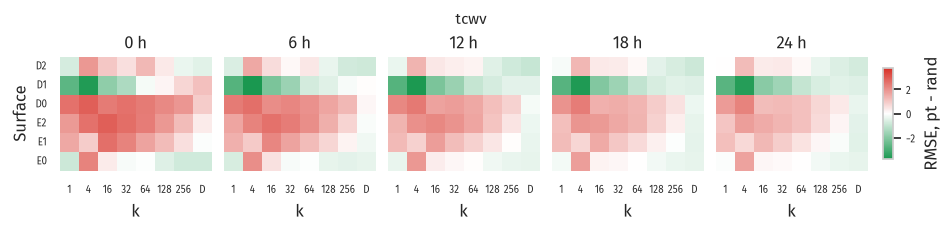
\includegraphics[width=\textwidth]{results/probe_heatmap_tcwv.png}\par
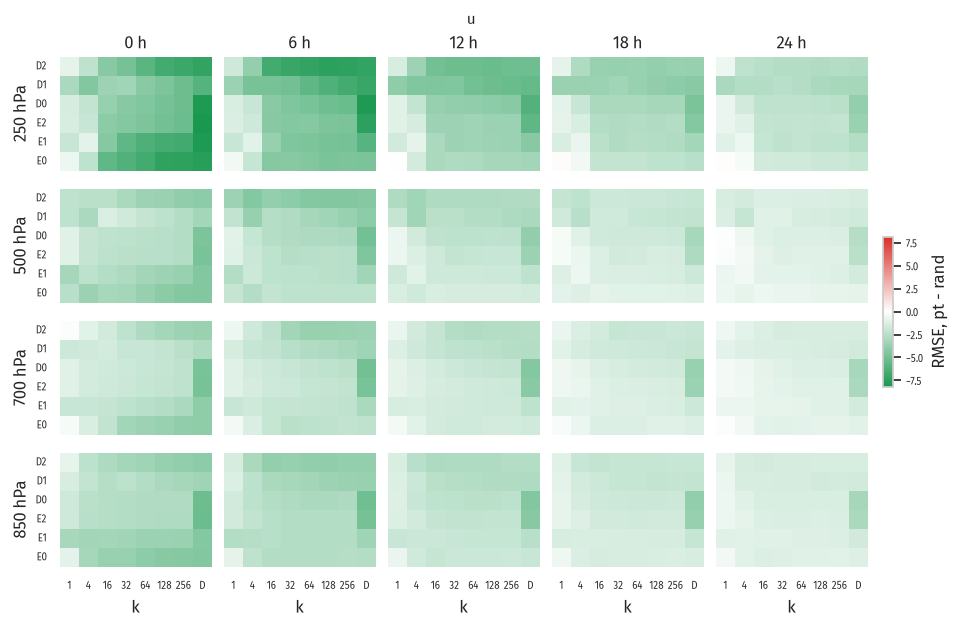
\includegraphics[width=\textwidth]{results/probe_heatmap_u.png}
\caption{Probe RMSE differences (pretrained -- random) for msl, tcwv, and u across backbone stages, channel counts $k$, and lead times. Negative (red) values indicate lower RMSE for probes trained on pretrained model activations.}
\label{fig:probe_heatmaps}
\end{figure*}

\section{Discussion}

\section{Conclusion}

\section*{Impact Statement}

\bibliography{bibliography,manual_bibliography}
\bibliographystyle{icml2026}

\newpage
\appendix
\onecolumn
\section{Additional Details}
\label{app:details}

\end{document}
